\documentclass[25pt]{sciposter}

\usepackage[T1]{fontenc}
\usepackage[utf8]{inputenc}

\usepackage{amsthm}

\usepackage[dvipsnames,usenames,svgnames,table]{xcolor} 
\usepackage{lipsum}
\usepackage{epsfig}
\usepackage{amsmath}
\usepackage{amssymb}
\usepackage[english]{babel}
\usepackage{geometry}
\usepackage{multicol}
\usepackage{graphicx}
\usepackage{tikz}
\usepackage{wrapfig}
\usepackage{gensymb}
\usepackage{tocloft}
\usepackage{empheq}

\usepackage{pgfplots}
\pgfplotsset{width=11cm,compat=1.9}


% for nice tableas
\usepackage{booktabs}

\graphicspath{ {img/} }

\geometry{
	landscape,
	a1paper,
	left=5mm,
	right=50mm,
	top=5mm,
	bottom=50mm,
}
\usepackage{array}   % for \newcolumntype macro
\newcolumntype{L}{>{$}m{5.5cm}<{$}} % math-mode version of "l" column type

%BEGIN LISTINGDEF





\newcommand*\widefbox[1]{\fbox{\hspace{2em}#1\hspace{2em}}}
\newcommand{\limm}{\lim\limits_{n \to \infty}}
\newcommand{\limx}[1]{\lim\limits_{x \to #1}}
\newlength\dlf  % Define a new measure, dlf
\newcommand\alignedbox[2]{
	% Argument #1 = before & if there were no box (lhs)
	% Argument #2 = after & if there were no box (rhs)
	&  % Alignment sign of the line
	{
		\settowidth\dlf{$\displaystyle #1$}
		% The width of \dlf is the width of the lhs, with a displaystyle font
		\addtolength\dlf{\fboxsep+\fboxrule}
		% Add to it the distance to the box, and the width of the line of the box
		\hspace{-\dlf}
		% Move everything dlf units to the left, so that & #1 #2 is aligned under #1 & #2
		\boxed{#1 #2}
		% Put a box around lhs and rhs
	}
}
\usepackage{graphicx,url}

%BEGIN TITLE
\title{\huge{Randomized Algorithms and Probabilistic Methods}}

\author{\large{David Zollikofer}}
%END TITLE

\usepackage{palatino}
%\usepackage{eulervm}
\usepackage{mathpazo}
% begin custom commands
\newcommand{\Q}{\mathbb{Q}}
\newcommand{\R}{\mathbb{R}}
\newcommand{\N}{\mathbb{N}}
\newcommand{\F}{\mathcal{F}}
\newcommand{\X}{\mathcal{X}}
\newcommand{\W}{\mathcal{W}}
\newcommand{\Nor}{\mathcal{N}}
\newcommand{\U}{\mathcal{U}}
\newcommand{\Var}{\operatorname{Var}}
\newcommand{\E}{\operatorname{E}}
%\newcommand{\exp}{\operatorname{exp}}

\newcommand{\mc}{\mathcal}

% some shortcuts
\newcommand{\ds}{\displaystyle}
\newcommand{\arr}{\rightarrow}
\newcommand{\nop}[1]{}
\renewcommand{\hat}{\widehat}

% stuff for integrals
\newcommand{\intl}{\int\limits}
\newcommand{\rmd}{\mathrm{d}}


\newcommand{\norm}[1]{\left\lVert#1\right\rVert}
\usepackage[framemethod=TikZ]{mdframed}
\newenvironment{method}[1]{\begin{mdframed}[backgroundcolor=blue!10,innertopmargin=15pt, innerbottommargin=15pt,nobreak=true]
		\textbf{#1 }
	}
	{ 
	\end{mdframed}
}

\newenvironment{important}{\begin{mdframed}[backgroundcolor=red!50,innertopmargin=15pt, innerbottommargin=15pt, nobreak=true]
		\Large
	}
	{ 
	\end{mdframed}
}

\newenvironment{lemma}{\begin{mdframed}[backgroundcolor=gray!50,innertopmargin=15pt, innerbottommargin=15pt, nobreak=true]
		\Large
	}
	{ 
	\end{mdframed}
}

\newenvironment{thm}[1]{\begin{mdframed}[backgroundcolor=pink!20,innertopmargin=15pt, innerbottommargin=15pt, nobreak=true]
		\textbf{#1 }
	}
	{ 
	\end{mdframed}
}



\newenvironment{defn}[1]{\begin{mdframed}[backgroundcolor=PineGreen!20,innertopmargin=15pt, innerbottommargin=15pt, nobreak=true]
		\textbf{#1 }
	}
	{ 
	\end{mdframed}
}


\usepackage{todonotes}
\newcommand{\TODO}[1]{\todo[inline]{\Large TODO:  #1}}





\DeclarePairedDelimiter\abs{\left|}{\right|}%



\setlength\abovedisplayskip{0pt}

\renewcommand{\familydefault}{\rmdefault}

% end custom commands

\begin{document}
	
	
	
	
	
	\maketitle
	
	
	
	\begin{multicols}{3}
		
		\section{Linearity of Expectation}
		
\begin{method}{Expectation Rules}
	For $X$ a random variable for which $\sum_{x\in W_X} |x| \Pr[X = x]$ converges 
	We have:
\begin{align*}
	\E[X] :&= \sum_{x\in W_x}^{x\cdot \Pr[X=x]}\\
	\E[X] &= \sum_{i=1}^{\infty} \Pr[X \geq i]
\end{align*}
\end{method}




			
		
		\section{The Inequalities of Markov and Chebychev}
		
		\begin{method}{Markov's Inequality}
			For $X$ a non-negative random variable, we have $\forall t > 0$
			\begin{align*}
				\Pr[X \geq t ]\leq \frac{\E[X]}{t}
			\end{align*}
		\end{method}
		
		
		\begin{method}{Chebychev's Inequality}
		For random variable $X$ and $\forall t > 0$ we have 
		\begin{align*}
			\Pr[|X-\E[X]| \geq  t] \leq \frac{\Var[X]}{t^2}
		\end{align*} 
	\end{method}

		\section{First \& Second Moment Method}
		
		\begin{method}{First Moment Method}
			Let $(X_n)_n$ be a sequence of random variables which take \textbf{non-negative integer values}. Then 
			\begin{equation}
				\E[X_n] = o(1) \implies \Pr[X_n = 0] = 1 - o(1)
			\end{equation}
		\end{method}
	
	\begin{method}{Second Moment Method}
		Let $(X_n)_n$ be a sequence of random variables. Then 
		\begin{align}
\E[X_n] \neq 0 \text{ ($n$ large) \& }& \Var[X_n] = o(\E[X_n]^2) \\
&\implies \Pr[X_n = 0] = o(1)
		\end{align}
	\end{method}
		
		
		
		\section{Chernoff Bounds}
	
\textbf{Chernoff Upper \& Lower Bounds}\\
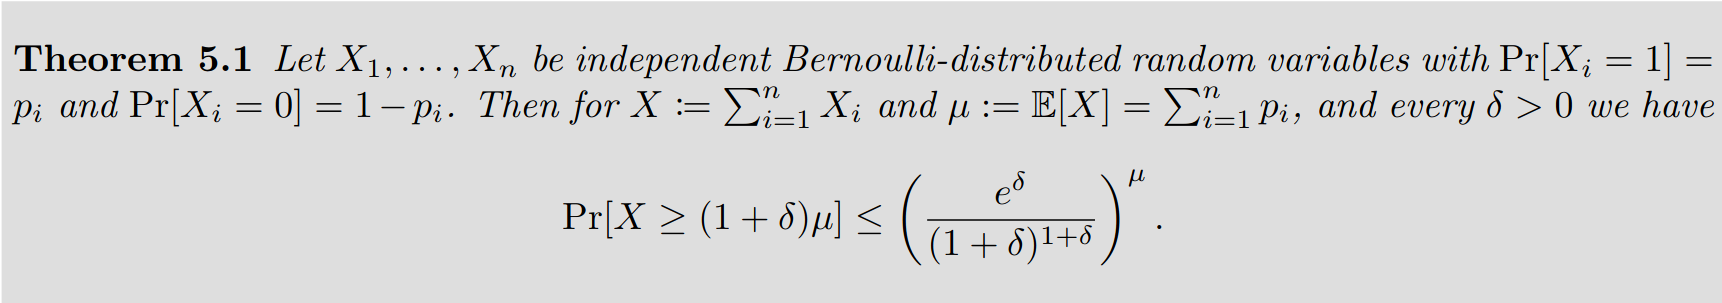
\includegraphics[width=\linewidth]{screenshot001}

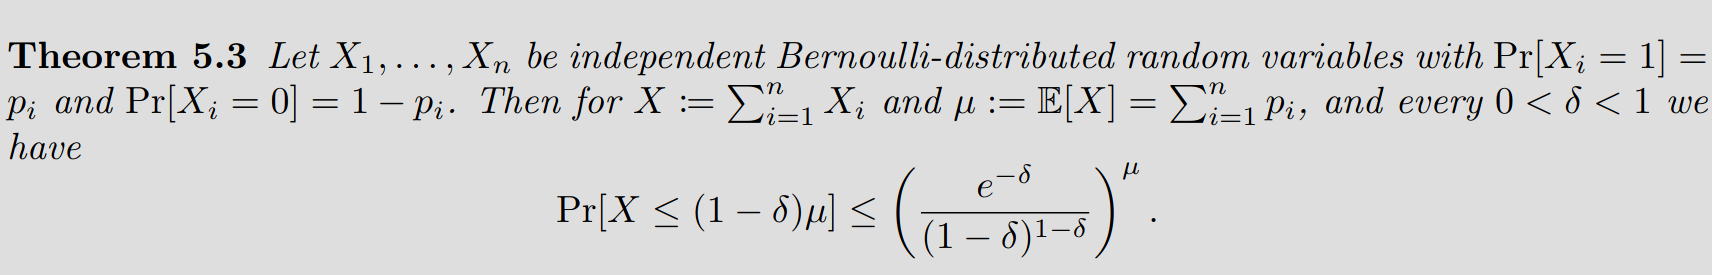
\includegraphics[width=\linewidth]{screenshot002}

\textbf{Chernoff Alternative Bounds}\\
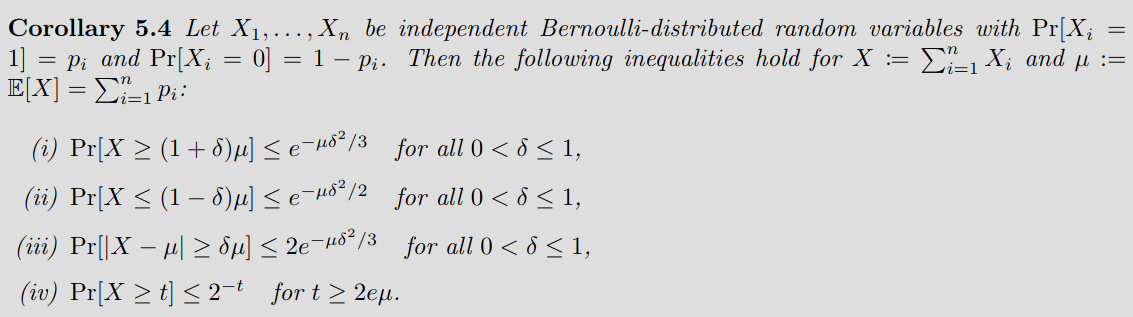
\includegraphics[width=\linewidth]{screenshot010}


\textbf{Chernoff Relaxation}\\
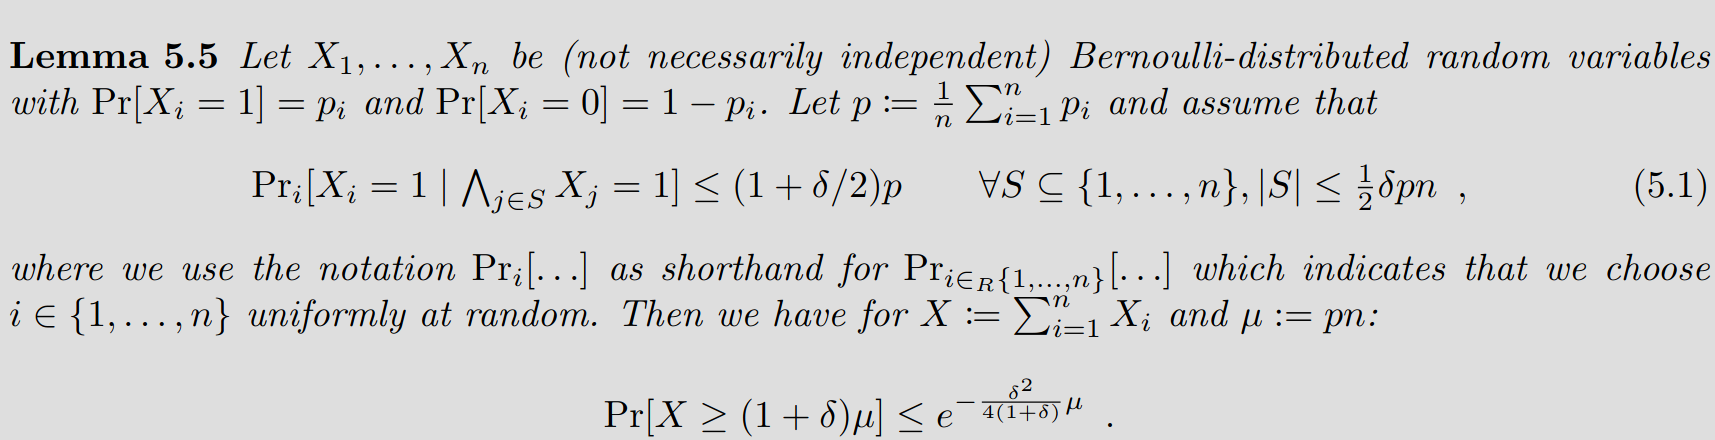
\includegraphics[width=\linewidth]{screenshot004}


		
		TODO print the cheatsheet randalg
		
		
		\textbf{Example (Routing in the Hypercube)} Every vertex $v$ chooses a random vertex $\sigma(v_i)$ to which the vertex sends using bit fixing. After $4d$ rounds the random vertex sends to original destination. 
		
		
		\section{Negative Correlation}
		
		\begin{method}{Negatively Correlated}
			Let $X_1, \ldots, X_n$ be Bernoulli random variables that are pairwise negatively correlated (i.e. $\E[X_i X_j] \leq\E[X_i] \cdot \E[X_j] $), then $X = \sum_{i=1}^{n} X_i$ satisfies
			\begin{align*}
				\Var[X] \leq \E[X]
				\end{align*}
		\end{method}
		It follows that the first and second moment method are very easy to apply
		\begin{thm}{Moment Methods Applied}
Let $(Z_n)_n$ be a sequence of random variables such that each $Z_i$ is the sum of of pairwise negatively correlated Bernoulli random variables then
\begin{align*}
	\E[Z_n] \to 0 &\implies \Pr[Z_n = 0] \to 1\\
	\E[Z_n] \to \infty &\implies \Pr[Z_n = 0] \to 0
\end{align*}
		\end{thm}	
	
	\begin{defn}{Negatively Associated}
	Random variables $X_1, \ldots, X_n$ are said to be negatively associated iff. for every two disjoint subsets $I,J \subseteq \{1,\ldots,n\}$ and every two functions $f:\R^{|I|} \to \R$ and $g:\R^{|J|} \to \R$ that are either both componentwise increasing or decreasing (not necessarily strictly) we have 
	\begin{align*}
		\E[f(X_i, i\in I) \cdot g(X_i, i\in J) ]\leq \E[f(X_i, i\in I)] \cdot \E[g(X_i, i\in J)]
	\end{align*}
	\end{defn}
	
	\begin{method}{Chernoff for Negatively Associated}
		The Chernoff bounds also hold or negatively associated random variables.
	\end{method}

\begin{method}{Bernoulli Negatively Associated}
	For $X_1, \ldots, X_n$ Bernoulli random variables with $\sum_{i=1}^{n} X_i \equiv 1$ the variables $X_1,\ldots, X_n$ are negatively associated.
\end{method}

	
	
		\section{Inequalities of Azuma and Jansson}
	
		\begin{defn}{Effect}
The effect of the $i$-th coordinate is given by $\max |X(\omega) - X(\omega')| $ for $\omega \in \Omega$
		\end{defn}
	
			\begin{method}{Azuma's Inequality}
				For $(\Omega, Pr)$ a product of the probability spaces $(\Omega_1, Pr_1) \cdots (\Omega_N, Pr_N)$ and $X;\Omega \to \R$ a random variable whose $i$-th coordinates effect is bound by $c_i$ we have
				\begin{align*}
					\Pr[X\geq \E[X] + t] &\leq e^{-\frac{t^2}{2\sum_{i=1}^{N} c_i ^2}}\\
					\Pr[X\leq \E[X] - t] &\leq e^{-\frac{t^2}{2\sum_{i=1}^{N} c_i ^2}}
				\end{align*}
			\end{method}	
				
			\begin{method}{Janson's Inequality}
See script page 58. 

\begin{align*}
	\Pr[X \leq \E[X] - t ] \leq e^{\frac{t^2}{2(\lambda + \Delta)}}
\end{align*}
\begin{align*}
	\Pr[X = 0 ] \leq e^{\frac{\lambda^2}{2(\lambda + \Delta)}} \leq e^{\min\{\lambda, \lambda^2 / \Delta\} / 4}
\end{align*}
where $\lambda = \E[X] = \sum_{i=1}^{m} \Pr[X_i = 1]$ and 

\begin{align*}
	\Delta := \sum_{i\neq j \land A_i \cap A_j \neq \emptyset} \Pr[X_i = 1 \land X_j = 1]
\end{align*}
these are all the summands of $\E[X^2]$ where we do not have independence of the two (but they also aren't the same).
			\end{method}
		
\section{Talagrand's Inequality}
\textbf{Talagrand's Inequality}\\
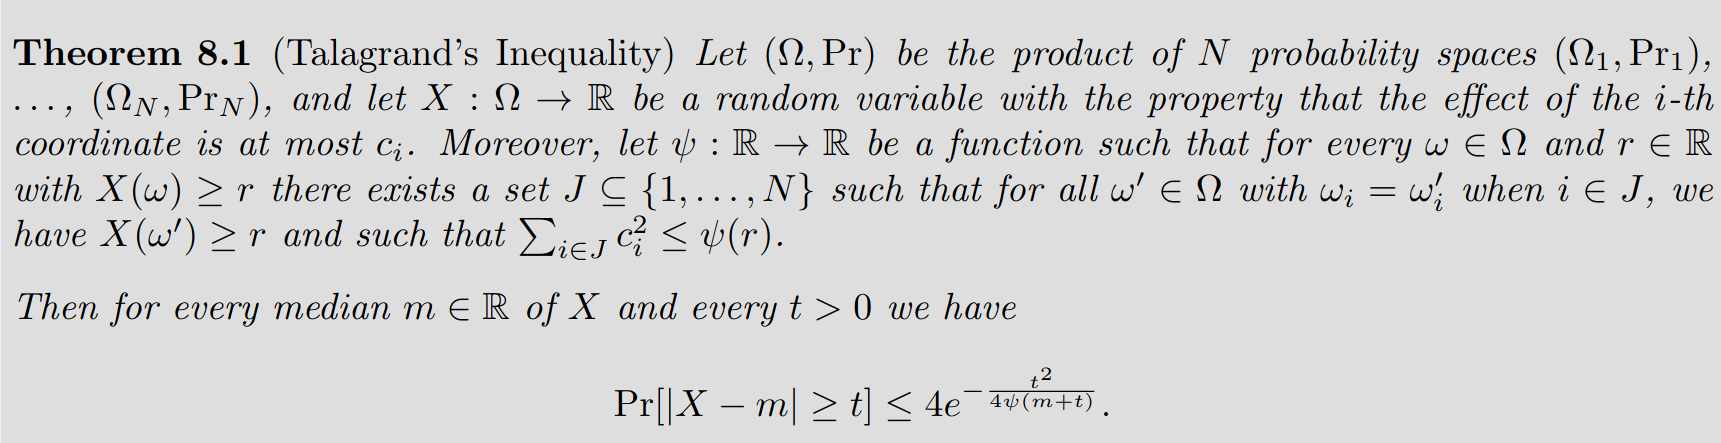
\includegraphics[width=\linewidth]{screenshot005.png}



\section{Drift Theorems}
\textbf{Additive}\\
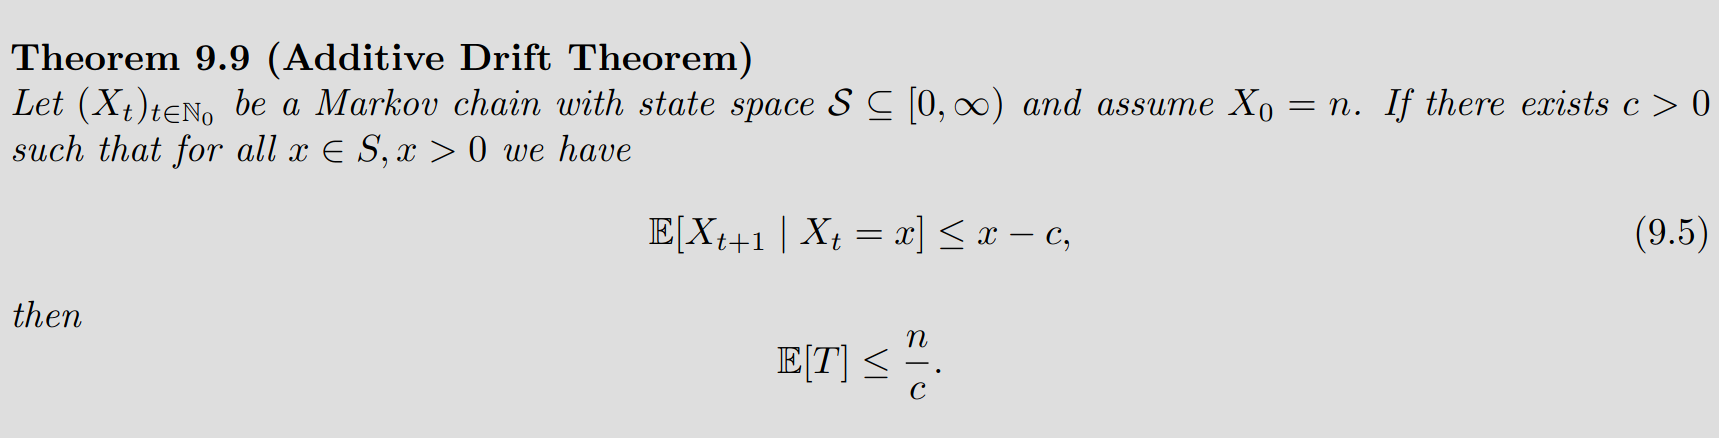
\includegraphics[width=\linewidth]{screenshot006}

\textbf{Additive with Injection}\\
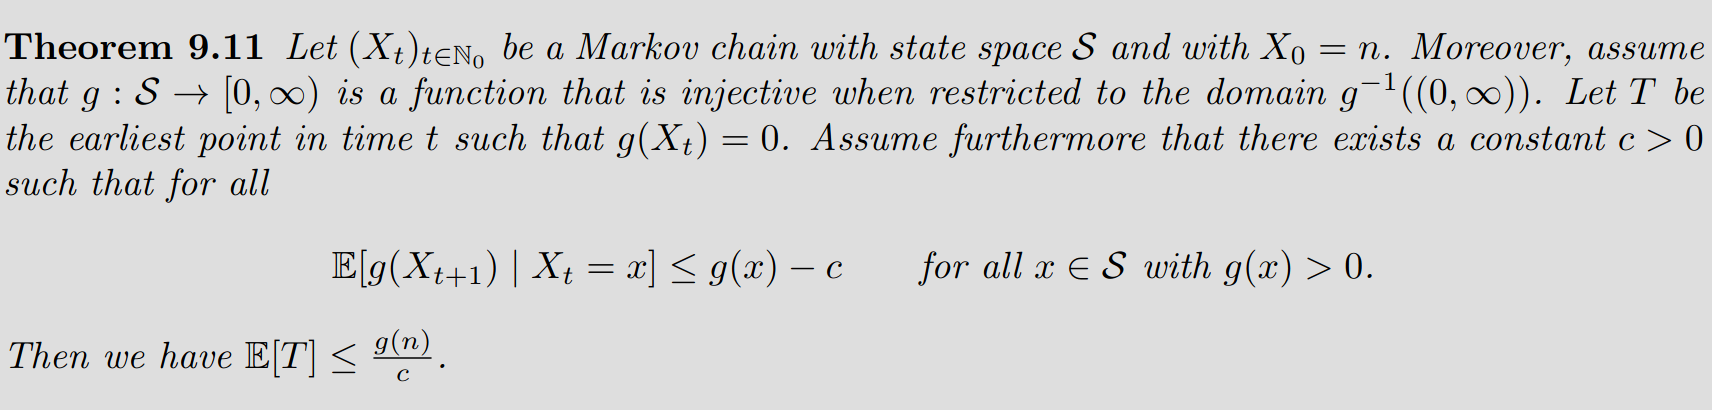
\includegraphics[width=\linewidth]{screenshot008}

\textbf{Multiplicative}\\
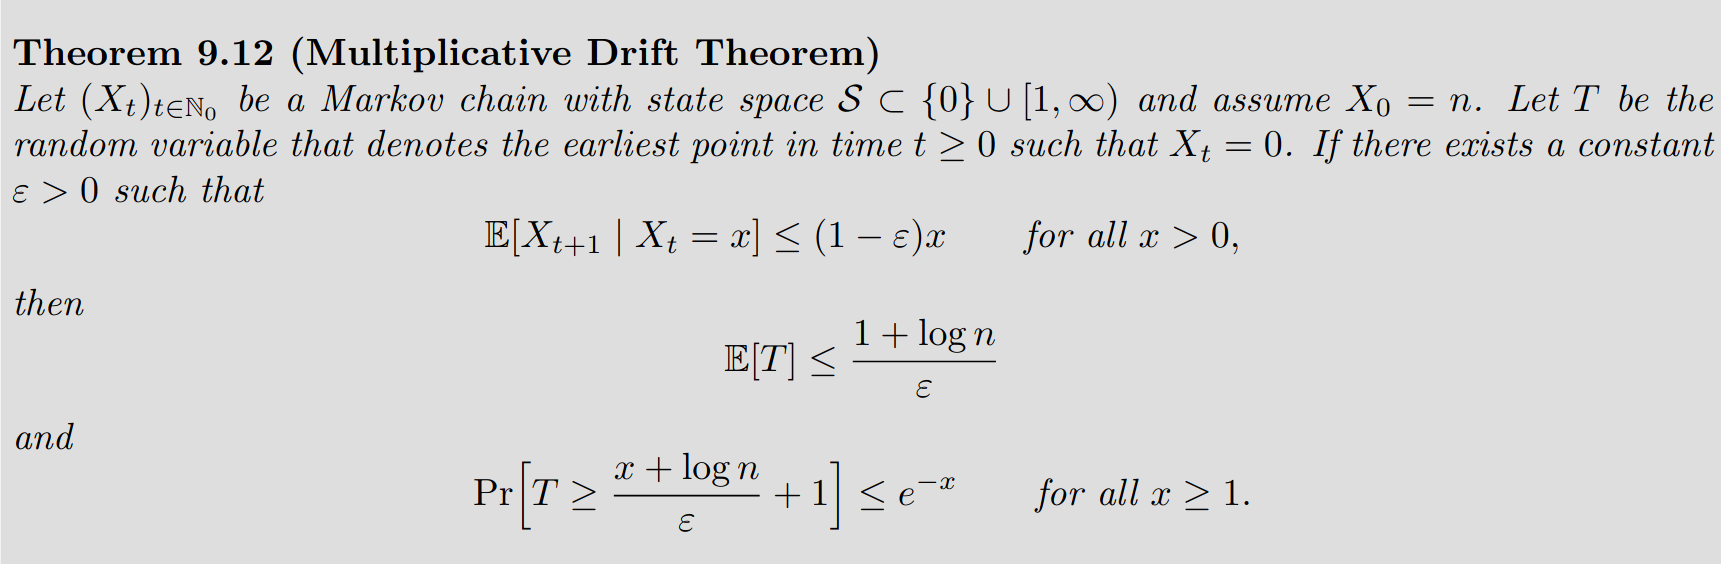
\includegraphics[width=\linewidth]{screenshot009}



		
		
		\section{Varia}
		\begin{defn}{Largest Independent Set}
Any vertex either is in the indepdendet set or has a neighbor in it. But no two neighboring vertixes may be in the independent set.
		\end{defn}
		
		\begin{defn}{Stirling's Approximation}
			
\begin{equation*}
	\ln(n!) = n \ln (n) -n + O(\ln n)
\end{equation*}
\begin{equation*}
	\sqrt{2\pi n} \left(\frac{n}{e}\right)^n e^{\frac{1}{12n + 1}} < n! < 	\sqrt{2\pi n} \left(\frac{n}{e}\right)^n e^{\frac{1}{12n}}
\end{equation*}
\end{defn}		
		

		
	
	
	
	
	
	
	
	
	\newpage
	
	
	
	
	
	
	
	
	
	
	
	
	
	
	
	

		
		
		
	\end{multicols}
\end{document}
